\documentclass[a4paper, 10pt]{report}
\usepackage{common}
\usetikzlibrary{petri,positioning}

% Cuerpo
\begin{document}

% Carátula
\title{
	II\\
	Programación Concurrente\\
	\large Clases 3 a 6: Memoria compartida
}
\author{Ramiro Martínez D'Elía}
\date{2021}
\maketitle

% Índice
\tableofcontents

\chapter{Locks y Barriers}
\vspace*{-10mm}

\section{Introducción}

Los programas concurrentes emplean dos tipos básicos de sincronización: exclusión mutua y sincronización por condición. Este capítulo examina 2 (dos) problemas importantes (secciones críticas y barreras).

El problema de la sección crítica se preocupa en implementar acciones atómicas por software. Este problema surge en la mayoría de los programas concurrentes, donde, la exclusión mutua es implementada mediante locks que protegen las secciones críticas.

Una barrera (barrier), es un punto de sincronización al que todos los procesos deben llegar, antes de que cualquier proceso se le permita proceder. Es un problema muy común en los programas paralelos.

\section{El problema de la sección crítica}

En este problema, \textbf{\emph{n}} procesos repetidamente ejecutan secciones críticas y no cŕiticas de código. La sección crítica está precedida por un protocolo de entrada y seguida por un protocolo de salida. Los procesos que contengan secciones críticas, deberían ser de la siguiente forma.

\begin{lstlisting}
Process SeccionCritica[i = 1 to n]
	while (true)
	   # Entry protocol
	   # critical section
	   # Exit protocol
	   # Noncritical section
	end;
 end;
\end{lstlisting}

Cada sección crítica, es un conjunto de sentencias que acceden a algún recurso compartido. Mientras que, cada sección no crítica es otra secuencia de instrucciones. Para resolver este problema, es necesario implementar protocolos de entrada y salida que cumplan las siguiente 4 (cuatro) propiedades:

\begin{enumerate}
	\item \textbf{Exclusión mutua:} A lo sumo un proceso podrá estar ejecutando su sección crítica. Esta es una \textbf{\emph{propiedad de seguridad}}; donde lo malo que puede ocurrir es que 2 (dos), o más, procesos accedan a su sección crítica en el mismo momento.
	\item \textbf{Ausencia de deadlock:} Si 2 (dos) o más procesos intentan entrar a sus secciones críticas, al menos uno tendrá éxito. Esta es una propiedad \textbf{\emph{propiedad de seguridad}}; donde lo malo que puede ocurrir es que todos los procesos estén esperando ingresar pero, ninguno sea capaz de lograrlo.
	\item \textbf{Ausencia de demoras inecesarias:} Si un proceso intenta ingresar a su sección crítica y los demás procesos se encuentran ejecutando sus secciones no críticas o finalizaron, el primer proceso no debe estar impedido de ingresar a su sección crítica. Esta es una \textbf{\emph{propiedad de seguridad}}, donde lo malo que puede ocurrir es que; un proceso no pueda ingresar a su sección crítica aunque no haya procesos en sus secciones críticas.
	\item \textbf{Eventual entrada:} Todo procesos que intente ingresar a su sección crítica, eventualmente lo logrará. Esta es una \textbf{\emph{propiedad de vida}} y es afectada directamente por la política de scheduling.
\end{enumerate}

Cualquier solución al problema de la sección crítica, también puede ser utilizada para implementar sentencias \textbf{\emph{await arbitrarias}}.

\section{Señalizando con barreras}

Varios problemas pueden ser resueltos utilizando algoritmos iterativos que sucesivamente computen aproximaciones a la respuesta. Terminando cuando la respuesta final haya sido procesada, o bien, haya convergido.

La idea es utilizar múltiples procesos, para procesar partes disjuntas de una solución en paralelo. La clave principal en la mayoría de los algoritmos paralelos, es que cada iteración depende del resultado de una iteración previa. Así, podemos llegar a la siguiente forma general para todo algoritmo que implemente barreras.

\begin{lstlisting}
Process Worker[i = 1 .. n]
	while (true)
	   # Realiza la tarea i
	   # Espera por los demas procesos
	end;
 end;
\end{lstlisting}

Esto es llamado sincronización por barrera, porque la demora al final de cada iteración representa una barrera a la cual todos los procesos deben llegar, antes de que a cualquier otro se le permita continuar.

\subsection{Barreras simétricas}

Si todos los procesos ejecutan el mismo algoritmo y cada proceso está ejecutando en un procesador distinto. Entonces, todos los procesos deberían llegar a la barrera casi al mismo tiempo.

Esta es la opción más adecuada para programas que ejecuten en máquinas con memoria compartida. Mas adelante, se abordarán algoritmos para este tipo de barreras; el \textbf{\emph{butterfly}} y \textbf{\emph{dissemination barrier}} más precisamente.

\subsection{Principio de sincronización por banderas}

Algunas soluciones, como \textbf{\emph{flags and coordinators}}, implementan este principio de sincronización. El cual, se basa en las siguientes premisas:

\begin{enumerate}
	\item El proceso que espera por un flag de condición, es el único que puede limpiar dicho flag.
	\item Un flag no puede ser activado, nuevamente, hasta no ser "limpiado".
\end{enumerate}

\chapter{Soluciones con variables compartidas}
\vspace*{-10mm}

\section*{Introducción}

La sincronización, en esta sección, será implementada mediante la técnica de \textbf{\emph{busy waiting}}. Donde un proceso evalúa, repetidas veces, una condición hasta que esta se vuelva verdadera.

\textbf{Ventajas}
\begin{enumerate}
	\item Puede ser implementada utilizando instrucciones, de máquina, disponibles es cualquier procesador moderno.
	\item Adecuada si cada proceso se ejecuta en su propio procesador.
\end{enumerate}

\textbf{Desventajas}
\begin{enumerate}
	\item Ineficiente en arquitecturas monoprocesador.
\end{enumerate}

\section{Para secciones críticas}

\subsection{Spin locks}

Solución de grano fino que utiliza instrucciones atómicas especiales, existentes en la mayoría de los procesadores. Por ejemplo, \textbf{\emph{Test and Set (TS)}}. Se dice que los procesos dan “vueltas” (spinning) hasta que se libere lock.

\begin{lstlisting}
bool lock = false;

Process CS[i = 1 to n]
	while (true)
		while (TS(lock)) skip;    # Entry
		# Critical Section
		lock = false;             # Exit
		# Noncritical Section
	end;
end;
\end{lstlisting}

\textbf{Ventajas}
\begin{enumerate}
	\item Cumple con 3 (tres) de los requisitos, para secciones críticas: \emph{garantiza exclusión mutua}, \emph{ausencia de deadlock} y \emph{ausencia de demoras inecesarias}.
\end{enumerate}

\textbf{Desventajas}
\begin{enumerate}
	\item La \emph{eventual entrada} se garantiza solo con \emph{schedulers fuertemente fairs}. Ya que lock se vuelve verdadera, con infinita frecuencia.
	\item No atiende prioridades, es decir; no controla el orden en que los procesos, demorados, entran a su sección crítica.
\end{enumerate}

\subsection{Implementaciones Fair}
\textbf{\emph{Spin locks}}, no termina siendo del todo adecuada. Sería deseable, contar con algoritmos que:
\begin{enumerate}
	\item Cumplan las 4 (cuatro) propiedades, de una sección crítica.
	\item Solo dependan de \emph{schedulers débilmente fair}.
	\item Sean más justos. Es decir, manejen prioridades.
\end{enumerate}

Los algoritmos \textbf{\emph{Tie breaker}}, \textbf{\emph{Ticket}} y \textbf{\emph{Bakery}} parecen más adecuados ya que, cumplen con todos los requisitos mencionados anteriormente.

\subsection{Tie breaker}

Este algoritmo asegura la exclusión mutua mediante dos variables, una por proceso, \lstinline{in1} e \lstinline{in2}. En caso de que ambas valgan verdadero (empate) emplea una variable adicional, \lstinline{last}, para determinar cuál fue el último en ingresar a su sección crítica.

\begin{lstlisting}
bool in1, in2 = false;
int last = 1;
\end{lstlisting}
\begin{lstlisting}[multicols=2, firstnumber=3]
Process CS1
	while (true)
		last = 1; in1 = true; # Entry
		while (in2 and last == 1) skip;
		# Critical Section
		in1 = false; #Exit
		# Noncritical Section
	end;
end;
	
Process CS2
	while (true)
		last = 2; in2 = true; # Entry
		while (in1 and last == 2) skip;
		# Critical Section
		in2 = false; # Exit
		# Noncritical section
	end;
end;
\end{lstlisting}

\textbf{Ventajas}
\begin{enumerate}
	\item No requiere instrucciones especiales.
	\item Prioriza al primer proceso, en iniciar el protocolo de entrada.
\end{enumerate}

\textbf{Desventajas}
\begin{enumerate}
	\item Dificil generalizarlo a \emph{n} procesos.
\end{enumerate}

\subsection{Ticket}

El algoritmo ticket, es una solución al problema de la sección crítica generalizada para \emph{n} procesos, fácil de entender e implementar. El algoritmo se basa en la entrega de tickets (números) a procesos y posteriormente atenderlos en orden de llegada.

Para esto, obligatoriamente, se requiere de alguna instrucción especial que entregue e incremente los números a cada proceso de forma atómica, para evitar duplicados. Esta instrucción puede ser \textbf{\emph{Fetch and Add}}. 

De no existir una instrucción máquina, de estilo \textbf{\emph{Fetch and Add}}, podemos reemplazarla con otra sección crítica.

\begin{lstlisting}
int number = 1;
int	next = 1; 
int[] turn[n] = ([n] 0);
\end{lstlisting}

\begin{lstlisting}[firstnumber=4, multicols=2]
# Con instruccion FA

Process Worker[i = 1..n]
	# Entry protocol
	turn[i] = FA(number, 1);
	while (turns[i] != next) skip;	
	# Critical Section
	next = next + 1;        # Exit
	# Noncritical Section
end;
# Sin instruccion FA

Process Worker[i = 1..n]
	turn[i] = number;
	<number = number + 1>
	while (turns[i] != next) skip;
	# Critical Section
	next = next + 1;
	# Noncritical Section
end;
\end{lstlisting}

\textbf{Ventajas}
\begin{enumerate}
	\item Sencillo de implemetar.
	\item General para \emph{n} procesos.
\end{enumerate}

\textbf{Desventajas}
\begin{enumerate}
	\item La implementación sin instrucciones especiales, puede entregar números repetidos. Esto, decrementa el grado de justicia del algoritmo.
\end{enumerate}


\subsection{Bakery}

Al igual que en el algoritmo ticket, los procesos obtienen un número y esperan a ser atendidos. La diferencia radica en que en el algoritmo bakery, cada proceso debe revisar el número de los demás para obtener uno mayor a todos los que se encuentran demorados.

\begin{lstlisting}
int[] turn[n] = ([n] 0);

Process SC [i = 1 .. n]
	while (true)
		turn[i] = 1; 
		turn[i] = max(turn) + 1;
		for (j = 1 to n st j != i)                              # Entry
			while (turn[j] != 0 and turn[i] > turn[j]) skip;
		# Critical Section
		turn[i] = 0;                                            # Exit
		# Noncritical Section
	end;
end;
\end{lstlisting}

\textbf{Ventajas}
\begin{enumerate}
	\item No requiere instrucciones especiales.
	\item General para \emph{n} procesos.
\end{enumerate}

\textbf{Desventajas}
\begin{enumerate}
	\item Resulta complejo, y costoso, calcular el máximo entre \emph{n} valores.
\end{enumerate}


\section{Para barreras}

\subsection{Shared counter}

La manera más sencilla de especificar una barrera, es la de utilizar un contador compartido iniciado en 0 (cero). 

Asumiendo que existan \emph{n} procesos que necesitan reunirse en un barrera. Cuando un proceso llega a la barrera, incrementa el contador; cuando el contador valga \emph{n}, todos los procesos podrán continuar.

\begin{lstlisting}
int count = 0;

Process Worker[i = 1 .. n]
	while (true)
		# Realizar tarea ...
		FA(count, 1);
		while (count != n) skip;
	end;
end;
\end{lstlisting}

\textbf{Ventajas}
\begin{enumerate}
	\item Solución adecuada para un \emph{n} pequeño.
\end{enumerate}

\textbf{Desventajas}
\begin{enumerate}
	\item La variable \emph{count} debe ser reiniciada cuando todos crucen la barrera y, por sobre todo, antes de que cualquier proceso intente incrementarla.
	\item Requiere instrucciones especiales.
	\item Requiere una política de administración eficiente. La variable \emph{count} es referenciada varias veces, esto puede provocar \textbf{\emph{Memory Contention}}.
\end{enumerate}

\subsection{Flags and coordinators}

El algoritmo utiliza \textbf{dos arreglos como flags}; el primero para marcar la llegada de cada proceso a la barrera. Y el segundo, para indicar a cada proceso que puede continuar. Este último arreglo es actualizado por un proceso coordinador.

\begin{lstlisting}[multicols=2]
int[] arrive[n] = ([n] 0);
int[] continue[n] = ([n] 0);

Process Worker[i = 1..n]
	while (true)
		# Realizar tarea
		arrive[i] = 1;
		while (continue[i] == 0) skip;
		continue[i] = 0;
	end;
end;
Process Coordinator
	while (true)
		for (i = 1 to n)
			while (arrive[i] == 0) skip;
			arrive[i] = 0;
		end;
		for (i = 1 to n)
			continue[i] = 1
	end;
end;
\end{lstlisting}

\textbf{Ventajas}
\begin{enumerate}
	\item Resetea correctamente los contadores.
	\item Evita \textbf{\emph{memory contention}}. Ya que, cada elemento del arreglo utiliza una línea de caché distinta.
\end{enumerate}

\textbf{Desventajas}
\begin{enumerate}
	\item El tiempo de ejecución del coordinador, es proporcional a \emph{n}. Por su uso, no es recomendable para \emph{n} muy grandes.
\end{enumerate}

\subsection{Combined tree barrier}
Este algoritmo combina el rol de los workers y el del coordinador, de forma tal que cada worker es, también, un coordinador.

Los procesos son organizados en forma de árbol y se procede con la siguiente lógica: cada nodo worker primero espera a que sus hijos le den la señal de llegada, luego avisa a su padre que él también llegó.

Cuando el nodo raíz, recibe la señal de llegada de sus hijos se sobreentiende que todos los demás workers también lo hicieron. Así, la raíz envía la señal de continuar a sus hijos y así sucesivamente.

\begin{lstlisting}
int[n] arrive = 0;
int[n] continue = 0;
\end{lstlisting}
\begin{lstlisting}[multicols=2, firstnumber=3]
Process Leaf[1..L]
	# Hacer algo ...
	arrive[L] = 1;
	< await (continue[L] == 1) >
	continue[L] = 0;
End.

Process Root
	< await(arrive[left] == 1) >
	arrive[left] = 0;
	< await(arrive[right] == 1) >
	arrive[right] = 0;
	# Hacer algo ...
	arrive[R] = 1;
	< continue[left] = 1;
	continue[right] = 1; >
End.
	
Process Internal[1..I]
	< await(arrive[left] == 1) >
	arrive[left] = 0;
	< await(arrive[right] == 1) >
	arrive[right] = 0;
	# Hacer algo ...
	arrive[I] = 1;
	< await(continue[I] == 1) >
	continue[I] = 0;
	< continue[left] = 1; 
	continue[right] = 1; >
End.
\end{lstlisting}

\textbf{Ventajas}
\begin{enumerate}
	\item Útil para \emph{n} muy grandes ya que, el tiempo de ejecución es proporcional al alto del árbol: $\log_2n$.
	\item Adecuado para máquinas con memoria distribuida.
\end{enumerate}

\subsection{Butterfly}
La idea es conectar barreras de pares de procesos, para construir una barrera de \emph{n} procesos. Asumiendo que \emph{Worker[1:n]} es un arreglo de procesos y que \emph{n} es potencia de 2, podríamos combinarlos de la siguiente manera.

Por la forma de conexión, es conocida como butterfly barrier. Como se aprecia en la figura, cada proceso se conecta con otro distinto en cada una de sus $\log_2n$ pasadas. Más precisamente, en cada pasada, cada proceso se sincroniza con otro a una distancia $2^{S-1}$.

Cuando un proceso finalizó todas sus pasadas, todos los procesos arribaron a la barrera y pueden proceder. Esto es, porque los procesos están directa o indirectamente sincronizados los unos con los otros.

\noindent
\begin{minipage}{.4\textwidth}
\begin{lstlisting}
int[n] arrive = 0;
int stages = log2(n);

Process Worker[i=1..n]
	for (s = 1 to stages)
		arrive[i] = arrive[i] + 1;
		j = neighbord_for(i, s);
		while (arrive[j] < arrive[i]) 
			skip;
	end;
End.
\end{lstlisting}
\end{minipage}
\noindent
\begin{minipage}{.6\textwidth}
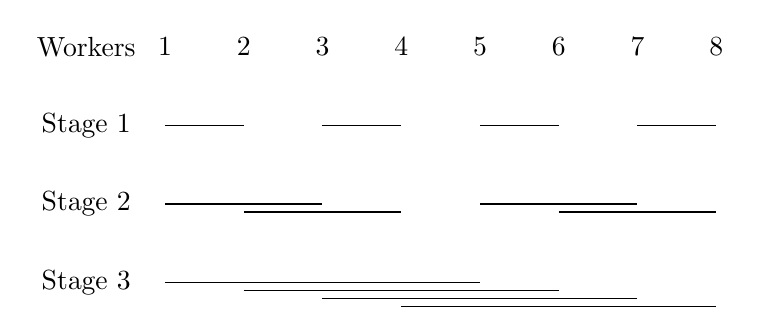
\begin{tikzpicture}
\node[] (label_w) at (0,0) {Workers};
\node[] (label_w1) at (1,0) {1};
\node[] (label_w2) at (2,0) {2};
\node[] (label_w3) at (3,0) {3};
\node[] (label_w4) at (4,0) {4};
\node[] (label_w5) at (5,0) {5};
\node[] (label_w6) at (6,0) {6};
\node[] (label_w7) at (7,0) {7};
\node[] (label_w8) at (8,0) {8};
\node[] (label_s1) at (0,-1) {Stage 1};
\node[] (label_s2) at (0,-2) {Stage 2};
\node[] (label_s3) at (0,-3) {Stage 3};
% Stage 1 barriers
\draw [line width = 0.5pt] (1,-1) -- (2,-1); % 1 con 2
\draw [line width = 0.5pt] (3,-1) -- (4,-1); % 3 con 4
\draw [line width = 0.5pt] (5,-1) -- (6,-1); % 5 con 6
\draw [line width = 0.5pt] (7,-1) -- (8,-1); % 7 con 8
% Stage 2 barriers
\draw [line width = 0.5pt] (1,-2) -- (3,-2); % 1 con 3
\draw [line width = 0.5pt] (2,-2.1) -- (4,-2.1); % 2 con 4
\draw [line width = 0.5pt] (5,-2) -- (7,-2); % 5 con 7
\draw [line width = 0.5pt] (6,-2.1) -- (8,-2.1); % 6 con 8
% Stage 3 barriers
\draw [line width = 0.5pt] (1,-3) -- (5,-3); % 1 con 5
\draw [line width = 0.5pt] (2,-3.1) -- (6,-3.1); % 2 con 6
\draw [line width = 0.5pt] (3,-3.2) -- (7,-3.2); % 3 con 7
\draw [line width = 0.5pt] (4,-3.3) -- (8,-3.3); % 4 con 8
\end{tikzpicture}
\end{minipage}%





Si \emph{n} no fuese potencia de 2, podría utilizarse el siguiente \emph{n} potencia de 2. Generando workers substitutos para cada iteración. Este workaround, decrementa la eficiencia del algoritmo.

\section{Defectos}

La mayoría de los protocolos implementados por \textbf{\emph{busy waiting}} son \textbf{\emph{complejos}} y la \textbf{\emph{separación entre variables}}, utilizadas para la sicronización y para cómputo general, es \textbf{\emph{poco clara}}.

Otro defecto es la \textbf{\emph{ineficiencia}} de los protocolos de busy waiting \textbf{\emph{en la mayoria de los programas multihilos}}. Excepto para el caso de los programas paralelos donde el número de procesos concuerde con el número de procesadores. 

No obstante, usualmente, existen más procesos que procesadores y \textbf{\emph{resulta menos productivo otorgar CPU a procesos para que hagan spinning en lugar de cómputo}}.

La eficiencia es fundamental, en los programas concurrentes, por esto es deseable tener herramientas más eficientes, para el desarrollo de aplicaciones concurrentes, como: \textbf{\emph{semáforos}} y \textbf{\emph{monitores}}. 

Con este tipo de herramientas, los procesos demorados no ocupan tiempo CPU hasta que no tengan la posibilidad de ejecutarse. En cuyo caso, serán colocados en una cola de listos.

\chapter{Soluciones con semáforos}
\vspace*{-10mm}

Al igual que los semáforos viales sirven para proveer un mecanismo de señalización para prevenir accidentes. En los programas concurrentes, los semáforos sirven para proveer un mecanismo de señalización entre procesos e implementar exclusión mutua y sincronización por condición.

\section{Sintáxis y semántica}

Un semáforo es una variable compartida, que puede pensarse en términos de una instancia de la clase semáforo. Dicha clase, posee solo dos métodos y una variable interna contador. 

El método \textbf{\emph{v}} es utilizado para señalar la ocurrencia de un evento, y en consecuencia incrementa de forma atómica el contador interno.

El método \textbf{\emph{p}}, demora al proceso hasta que un evento haya ocurrido y decrementa de forma atómica el contador interno.

Por último, el \textbf{\emph{contador}} es una variable que sólo toma valores enteros positivos.



\begin{multicols}{2}

	%== Multicols no soporta table ... ==%
	{\renewcommand{\arraystretch}{2}%
	\centering
	\begin{tabular}{cc}
		\textbf{Tipo de semáforo} & \textbf{Valores del contador}\\
		\hline 
		Binario & Entre 0 y 1\\ 
		General & Entre 0 y $\infty$\\ 
	\end{tabular}}

\begin{lstlisting}
sem s;

P(s): < await(s > 0) s = s - 1; >

V(s): < s = s + 1; >
\end{lstlisting}

\columnbreak


	
\end{multicols}




\subsection{Para secciones críticas}

El problema de la sección crítica se puede resolver empleando una variable \emph{lock}. La cual, valdrá 1 (\emph{true}) si no hay procesos en su sección crítica ó 0 (\emph{false}) en caso contrario.

Cuando un proceso desea entrar en su sección crítica; primero deberá esperar a que lock valga 1 (\emph{true}) y luego colocar lock en 0 (\emph{false}). Cuando un proceso sale, deberá colocar a lock nuevamente en (\emph{true}).

\begin{lstlisting}
sem mutex = 1;
Process SC[i = 1 .. n]
	while (true)
		P(mutex);     # Entry
		# Seccion Critica
		V(mutex);     # Exit
		# Seccion no critica
	end;
end;
\end{lstlisting}

\section{Split Binary Semaphores}

La técnica split binary semaphores consiste en combinar 2 (dos), o más, semáforos binarios como si fuesen un solo. Todo conjunto de semáforos, formaran un SBS si cumplen la siguiente regla: $0 \leq s_{1} + s_{2} + ... + s_{n} \leq 1$.

\subsection{Productores y consumidores}

Dado un programa donde los procesos se comunican, entre sí, mediante un \textbf{\emph{búffer con capacidad para 1 (un) mensaje}}. En dicho programa, existiran 2 (dos) clases de procesos: los productores y los consumidores. Los \textbf{\emph{productores}}; crean mensajes, esperan a que el búffer esté vacío, depositarán su mensaje y marcarán el búffer como lleno. Mientras que, los \textbf{\emph{consumidores}}; esperan a que el búffer esté lleno, retiran el mensaje y marcan el búffer como vacío.

La forma más sencilla de sincronizar a los procesos es; utilizar semáforos en terminos de los estados posibles del búffer; \emph{empty} y \emph{full}. Juntos, \emph{empty} y \emph{full}, conforman un split binary semaphore que; proveerá exclusión mutua sobre el acceso del búffer.

\begin{lstlisting}
sem empty = 1, full = 0;
any buffer;
\end{lstlisting}
\begin{lstlisting}[multicols=2, firstnumber=3]
Process Consumer[1..n]
	while (true)
		P(full);
		message = buffer;
		V(empty);
	end;
End.

Process Producer[1..n]
	while (true)
		P(empty);
		buffer = message;
		V(full);
	end;
End.
\end{lstlisting}

\section{Contadores de recursos}

Usualmente los procesos compiten por el acceso a recursos limitados. En esos casos, \textbf{\emph{semáforos generales}}; pueden ser utilizados como contadores de recursos disponibles.

\subsection{Buffers limitados}

Dado un programa donde los procesos se comunican, entre sí, mediante un \textbf{\emph{búffer con capacidad para n mensaje}}. En dicho programa, existiran 2 (dos) clases de procesos: los productores y los consumidores. Los \textbf{\emph{productores}}; crean mensajes, esperan a que el búffer esté vacío, depositarán su mensaje y marcarán el búffer como lleno. Mientras que, los \textbf{\emph{consumidores}}; esperan a que el búffer esté lleno, retiran el mensaje y marcan el búffer como vacío.

En este caso, el recurso son los espacios libres del buffer. Como adición, se debe aplicar exclusión mutua para que distintos consumidores no recuperen el mismo mensaje (mantener consitente \emph{front}) y para, que los productores no sobreescriban mensajes (mantener consistente \emph{near}).

\begin{lstlisting}
int front, rear = 0;
sem empty = n, full = 0;
sem mutexFetch = 1, mutexDeposit = 1;
array[n] buffer; 
\end{lstlisting}
\begin{minipage}{\linewidth} % Avoid page break
\begin{lstlisting}[multicols=2, firstnumber=5]
Process Producer[1..n]
	while (true)
		P(empty); 
		P(mutexDeposit);
		buffer[rear] = data;
		rear = (rear + 1) % n;
		V(mutexDeposit); 
		V(full);
	end;
End.
Process Consumer[1..n]
	while (true)
		P(full);
		P(mutexFetch)
		data = buffer[front];
		front = (front + 1) % n;
		V(mutexFetch)
	end;
End.
\end{lstlisting}	
\end{minipage}


\section{Exclusión mutua selectiva}

La exlusión mutua selectiva, se presenta cuando cada proceso compite contra un subconjunto de procesos (por un recurso). En lugar de, competir contra todos.

\subsection{Dining Philosophers}

Por ejemplo: cinco filósofos se sientan a comer en una mesa redonda donde hay solo cinco tenedores. Cada filósofo, para comer, requiere de dos tenedores. Esto implica que; dos filósofos vecinos no pueden comer al mismo tiempo y que, a lo sumo, solo dos filósofos podrán comer al mismo tiempo.

El problema de exclusión mutua selectiva se da entre cada par de filósofos y un tenedor. Tener en cuenta, de que si fuesen 3 filósofos, no sería un problema de exclusión mutua.


\begin{lstlisting}[multicols=2]
sem forks[5] = {0,0,0,0,0}

Process Philosopher[i = 0 to 3]
	while(true)
		p(fork[i]);
		p(fork[i+1]);
		# come ...
		v(fork[i]); 
		v(fork[i+1]);
	end;
end;

Process Philosopher[4]
	while(true)
		p(fork[0]);
		p(fork[4]);
		# come ...
		v(fork[0]); 
		v(fork[4]);
	end;
end;
\end{lstlisting}

\begin{basic_box}
	\faIcon[regular]{gem} Si en lugar de 5 filósofos fueran 3, ¿el problema seguiría siendo de exclusión mutua selectiva? ¿Por qué?

	Si hay 3 filósofos, por consiguiente hay 2 tenedores. Lo que significa que todos los procesos son adyacentes, por lo cual la competencia se da entre todos y dejaría de ser un problema de exclusión mutua selectiva.
\end{basic_box}
\begin{basic_box}
	\faIcon[regular]{gem} El problema de los filósofos resuelto de forma centralizada y sin posiciones fijas ¿es de exclusión mutua selectiva? ¿Por qué?

	Si los filósofos pueden utilizar cualquier cubierto (sin posiciones fijas) y, en caso de haber disponibilidad, son servidos por un mozo (coordinador). No estamos hablando de exclusión mutua selectiva ya que, los filosofos compiten contra todos no solo contra sus adyacentes.
\end{basic_box}

\subsection{Lectores y escritores}

Otro ejemplo, de exclusión mutua selectiva, donde clases de procesos, compiten por el acceso a un recurso es el siguiente. Procesos escritores, que requieren acceso exclusivo para evitar interferencias. Y procesos, lectores, los cuales pueden acceder de forma concurrente entre sí (siempre y cuando no haya escritores haciendo uso de la base de datos).

El siguiente algoritmo, resuelve el problema. No obstante, esta solución no es fair. Ya que, prioriza lectores por sobre escritores.

\begin{lstlisting}
int nr = 0; # lectores activos
sem rw = 1; # acceso a bbdd
sem mutexR = 1; # acceso a nr
\end{lstlisting}
\noindent
\begin{minipage}{0.5\textwidth}
\begin{lstlisting}[firstnumber=4]
Process Reader
	while (true)
		P(mutexR)
		nr = nr + 1;
		if (nr == 1) P(rw);
		V(mutexR);
		# lee en bbdd
		P(mutexR)
		nr = nr - 1;
		if (nr == 0) V(rw);
		V(mutexR);
	end;
end;
\end{lstlisting}
\end{minipage}
\noindent
\begin{minipage}{0.5\textwidth}
\begin{lstlisting}[firstnumber=17]
Process Writer
	while (true)
		P(rw);
		# escribe en bbdd
		V(rw);
	end;
end;
\end{lstlisting}
\end{minipage}
\begin{basic_box}
	\faIcon[regular]{gem} Si solo se acepta sólo 1 escritor  o 1 lector en la BD, ¿tenemos un problema de exclusión mutua selectiva? ¿Por qué?

	En este caso, sería solo un problema de exclusión mutua. Debido a que, por definición, la competencia es entre todos los procesos (lectores vs escritores, lectores vs lectores, escritores vs escritores).
\end{basic_box}

\section{Passing the Baton}

Técnica que utiliza \textbf{\emph{split binary semaphores}} para proveer exclusión mutua y despertar procesos demorados (incluso respetando su orden). Empleando esta técnica, podremos \textbf{\emph{especificar sentencias await arbitrarias}}. Su implementación, respeta la siguiente forma:

\begin{enumerate}
	\item Un semáforo \textbf{\emph{e}}. Inicialmente en 1 para, controlar los accesos a la sección crítica.
	\item Un semáforo \textbf{\emph{$b_j$}} para demorar procesos hasta que, su guarda, \textbf{\emph{$B_j$}} sea verdadera.
	\item Un contador \textbf{\emph{$d_j$}} para contar los procesos demorados por \textbf{\emph{$b_j$}}.
\end{enumerate}

Cuando un proceso se encuentra en su sección crítica, retiene el permiso de ejecución (\textbf{\emph{baton}}). Al finalizar, le pasa el permiso a otro proceso (si lo hubiera) o bien, lo libera.

\subsection{Lectores y escritores}

Resolveremos el mismo problema, de lectores y escritores, de la sección anterior introduciendo la técnica \textbf{\emph{passing the baton}}. Donde:

\begin{itemize}
	\item \textbf{\emph{e}} $\rightarrow$ \emph{e}
	\item \textbf{\emph{$b_j$}} $\rightarrow$ \emph{r} y \emph{w}
	\item \textbf{\emph{$d_j$}} $\rightarrow$ \emph{dr} y \emph{dw}
\end{itemize}

Si bien este algoritmo, sigue priorizando a los lectores; podremos modificar a \textbf{\emph{SIGNAL}} para darle la política que quisieramos.

\noindent
\begin{minipage}{\textwidth}
\begin{lstlisting}[multicols=2]
int nr = 0,  # Lectores activos
int nw = 0;  # Escritores activos
	
int dr = 0, # Lectores demorados
int dw = 0; # Escritores demorados

# SBS: 0<=(e+r+w)<=1
sem e = 1,  # Baton
sem r = 0,  # Demora lectores
sem w = 0;  # Demora escritores
SIGNAL:
	if (nw == 0 & nr > 0)
		dr--;
		V(r);
	elseif (nr == 0 & nw == 0 & dw > 0)
		dw--
		V(w);
	else
		V(e);
\end{lstlisting}
\begin{lstlisting}[multicols=2, firstnumber=20]
Process Writer[1..n]
	while (true)
		P(e);
		if (nr > 0 or nw > 0)
			dw++;
			V(e);
			P(w);
		end;
		nw++;
		SIGNAL
		# Escribir en la bbbd ...
		P(e);
		nw--;
		SIGNAL
	end;
End.

Process Reader[1..n]
	while (true)
		P(e);
		if (nw > 0)
			dr++;
			V(e);
			P(r);
		end;
		nr++;
		SIGNAL
		# Leer en la bbbd ...
		P(e);
		nr--;
		SIGNAL
	end;
End.
\end{lstlisting}
\end{minipage}

\begin{basic_box}
	\faIcon[regular]{gem} ¿Qué relación encuentra con la técnica de passing the condition?

	Ambas técnicas poseen la misma finalidad. Solo que, Passing the condition es utilizada en Monitores.
\end{basic_box}

\subsection{Alocación de recursos - SJN}

En los problemas de alocación de recursos, se deben implementar políticas de acceso generales a un recurso compartido por los procesos.

Dichas políticas deben contemplar: cuándo se le puede dar acceso a un proceso y cuál proceso toma el recurso si hubiese más de uno esperando.

Como su nombre lo indica, una política de \textbf{\emph{Short Job Next}} le otorga el recurso al proceso en espera con menor valor de tiempo (el más corto). Su semántica, es la siguiente:

\begin{itemize}
	\item \lstinline{request(time, id)}: Un proceso solicita el acceso. Si el recurso está libre, se le otorga. Caso contrario, se coloca al proceso en una lista de espera.
	\item \lstinline{release}: Un proceso libera el recurso. Si hay procesos en espera se otorga, el recurso, al proceso con valor de tiempo más chico. Caso contrario, el recurso queda libre.
\end{itemize}

Este problema puede ser implementado, utilizando la técnica Passing the baton de la siguiente manera:

\noindent
\begin{minipage}{0.5\textwidth}
\begin{lstlisting}
request(time, id):
	P(e);   # mutex sobre free
	if (not free) DELAY;
	free = false;
	SIGNAL;

release():
	P(e);   # mutex sobre free
	libre = true;
	SIGNAL;
\end{lstlisting}
\end{minipage}
\begin{minipage}{0.5\textwidth}
En \textbf{DELAY} un proceso:
\begin{itemize}
	\item Se coloca en una lista de espera.
	\item Libera SC ejecutando \lstinline{V(e)}.
	\item Demora en un semáforo \lstinline{b[id]}.
\end{itemize}

En \textbf{SIGNAL} un proceso:
\begin{itemize}
	\item Cuando se libera el recurso, se le asigna al próximo proceso en espera si lo hubiera.
\end{itemize}
\end{minipage}


Esta política minimiza el tiempo promedio de ejecución pero, \textbf{no es una solución fair}. Procesos con un tiempo mayor, pueden quedar relegados ante la aparición de procesos con tiempo menor. 

Dicha desventaja se puede evitar, implementando políticas de \textbf{aging}. Es decir controlando, también, el tiempo en el que un proceso estuvo en lista de espera.

\section{Instrucciones máquina utilizadas}

\subsection{Fetch and Add}
De manera atómica incrementa \emph{number} en \emph{inc} veces y retorna su antiguo valor.

\begin{lstlisting}
FA (int number, int inc)
	< int temp = number;
	number = number + inc;
	return temp; >
end;
\end{lstlisting}

\subsection{Test and Set}

De manera atómica setea \emph{lock} en true y retorna su antiguo valor.

\begin{lstlisting}
bool TS(bool lock)
	< bool initial = lock; 
	lock = true; 
	return initial; >
end;
\end{lstlisting}

\section{Desventajas}

Los semáforos resultan un mecanismo de sincronización fundamental. Con ellos, podemos resolver cualquier problema de sincronización.

No obstante, por naturaleza, son un mecanismo de bajo nivel. Un algoritmo que emplea semáforos posee las siguientes características que, pueden llevar a que el programador cometa errores.

\begin{itemize}
	\item Variables compartidas globales a los procesos.
	\item Protocolos de entrada a secciones críticas, dispersas en el código.
	\item Al agregar procesos, se debe verificar el acceso correcto a las variables compartidas.
	\item La implementación de exclusión mutua y sincronización por condicion son similares, aunque los conceptos sean distintos.
\end{itemize}

\chapter{Soluciones con Monitores}

\section{Introducción}

Los monitores son módulos, del programa, que ofrecen una estructura que permite desarrollar programas concurrentes más limpios con respecto al uso de semáforos.

Principalmente, los monitores, funcionan como una capa de abstracción de datos. Un monitor encapsula la representación de un objeto abstracto (o recurso) y ofrece un conjunto de operaciones para manipularlo.


\begin{tikzpicture}
	\node[] () at (0.5,0.5) {}; %space
	\node[] at (10,-1) {Procesos Concurrentes};
	\node[circle,draw, minimum size=1cm] (P0) at (0,-1) {$P_0$};
	\node[circle,draw, minimum size=1cm] (P1) at (2,-1) {$P_1$};
	\node[circle,draw, minimum size=1cm] (Px) at (4,-1) {$...$};
	\node[circle,draw, minimum size=1cm] (Pn) at (6,-1) {$Pn$};
	\draw (-1,-3) -- (7,-3) -- (7,-5) -- (-1, -5) -- cycle;
	\node[] at (10,-4) {Tipo de dato abstracto};
	\node[draw, fill=white](interface) at (3,-3) {Interface};
	\draw[thick] (P0) edge[post] (interface);
	\draw[thick] (P1) edge[post] (interface);
	\draw[thick] (Px) edge[post] (interface);
	\draw[thick] (Pn) edge[post] (interface);
	\node[ellipse,draw, minimum size=1cm] (SharedData) at (1, -4) {Shared Data};
	\node[ellipse,draw, minimum size=1cm] (SyncData) at (5, -4) {Sync Data};
\end{tikzpicture}


\section{Sintáxis y Semántica}

Un monitor es utilizado para agrupar la representación e implementación de un recurso compartido (class). La especificación de un monitor consta de las siguientes partes:

\begin{itemize}
	\item \textbf{Interface}: Especifica las operaciones provistas por el recurso.
	\item \textbf{Cuerpo}: Contiene las variables que representan al recurso y procedimientos que implemetan las operaciones de la interfaz.
\end{itemize}

\begin{lstlisting}
Monitor Example

# Declracion de variables permanentes.
# Inicializacion de variables.

procedure op_test(formals)
	# Body ...
end;
End.
\end{lstlisting}

Las \textbf{\emph{variables permanentes}} son compartidas por todos los procedimientos dentro del monitor. Son llamadas permanentes, porque existen y consevan sus valores durante todo el ciclo de vida de un monitor. Ellas son inicializadas antes de cualquier llamado a procedimientos.

Los \textbf{\emph{procedimientos}}, tienen acceso a las variables permanentes, parámetros formales y sus variables locales. Estas últimas, son copiadas e inicializadas en cada llamado al procedimiento.

La principal ventaja, del uso de monitores, es que pueden ser desarrollados de manera aislada al programa que los vaya a utilizar.

\section{Sincronización}

En monitores, a lo sumo \textbf{un procedimiento} puede estar \textbf{activo a la vez}. Un procedimiento se considera activo, cuando un proceso externo se encuentra ejecutando alguna de sus sentencias. 

De esta forma, la \textbf{\emph{exclusión mutua}} se garantiza de forma \textbf{implícita}. Esto hace los algoritmos más fáciles de leer ya que, no hay protocolos de entrada y salida explícitos.

En contraste, la \textbf{\emph{sincronización por condición}} debe ser especificada de forma \textbf{explícita}. Esto se debe a que, las condiciones son diferentes en cada programa.

\subsection{Variables condición}

Una variable condición es utilizada para demorar un proceso que no puede continuar ejecutandose, de forma segura, hasta que algún estado del minitor satisfaga una condición. 

También son usadas para despertar procesos demorados, cuando la condición se vuelva verdadera. 

Este tipo de variables, solo pueden ser utilizadas dentro de un monitor. Y su declaración, sigue la siguiente forma:

\begin{lstlisting}
cond vc;
\end{lstlisting}

Internamente el valor de \lstinline{vc} es el de una cola, inicialmente vacía. El programador no manipula directamente la cola, sino que lo hace mediante operaciones especiales.

\begin{itemize}
	\item \lstinline{empty}: Retorna \lstinline{true} si la cola está vacía. Retornará \lstinline{false}, en caso contrario.
	\item \lstinline{wait}: Causa la demora del proceso en ejecución y lo agrega a la cola.
	\item \lstinline{signal}: Despierta procesos demorados y los retira de la cola.
\end{itemize}

Si bien, es posible definir una política de prioridades a la cola de procesos demorados; el comportamiento por defecto es el de una política FIFO. De esta forma: \lstinline{wait} colocará procesos al final de la cola y \lstinline{signal} desperatá al proceso que este en el frente.

\section{Disciplinas de señalización}

Cuando un proceso ejecuta \lstinline{signal}, se encuentra dentro de un monitor y por consiguiente tiene el control del lock implícito asociado al monitor. 

Dicha situación plantea un dilema. Si \lstinline{signal} despierta a otro proceso, ahora tendremos 2 (dos) procesos ejecutandose dentro del monitor y por definición, solo un proceso debe tener acceso exclusivo al monitor.

Ante la situación planteada, podemos adoptar alguna de las siguientes políticas:

\begin{enumerate}
	\item \textbf{\emph{Signal and Continue (SC)}}: El proceso \emph{señalizador} continua su ejecución. El proceso \emph{señalizado}, es colocado en la cola de listos y espera a que se libere el monitor para continuar.
	\item \textbf{\emph{Signal and Wait (SW)}}: El proceso \emph{señalizado} continua su ejecución. El proceso \emph{señalizador}, espera a que se libere el monitor para continuar.
\end{enumerate}

\section{Sincronización básica por condición}

\subsection{Buffers limitados}

\begin{itemize}
	\item \lstinline{not_full} $\rightarrow$ señaliza \lstinline{count < n}
	\item \lstinline{empty} $\rightarrow$ señaliza \lstinline{count > 0}
\end{itemize}

\begin{lstlisting}
monitor BoundedBuffer

typeT buffer[n];
int front = 0, rear = 0, count = 0;
cond not_full, not_empty;
\end{lstlisting}

\noindent
\begin{minipage}{0.5\textwidth}
\begin{lstlisting}[firstnumber=6]
procedure deposit(typeT data)
	while(count == n) wait(not_full);
	buffer[rear] = data;
	rear = (rear + 1) % 10;
	count++;
	signal(not_empty)
end;
\end{lstlisting}
\end{minipage}
\begin{minipage}{0.5\textwidth}
\begin{lstlisting}[firstnumber=13]
procedure fetch(typeT &result)
	while(count == 0) wait(not_empty);
	result = buffer[front];
	front = (front + 1) % n;
	count--;
	signal(not_full);
end;
\end{lstlisting}
\end{minipage}

\section{Broadcast}

\subsection{Lectores y Escritores}

\begin{itemize}
	\item \lstinline{oktoread} $\rightarrow$ señaliza \lstinline{nw == 0}
	\item \lstinline{oktowrite} $\rightarrow$ señaliza \lstinline{nw == 0 && nr == 0}
	\item \lstinline{signal_all} $\rightarrow$ despierta a todos (broadcast)
\end{itemize}

\begin{lstlisting}
monitor RW_Controller

int nr = 0, nw = 0;
cond oktoread, oktowrite;
\end{lstlisting}
\noindent
\begin{minipage}{0.5\textwidth}
\begin{lstlisting}[firstnumber=5]
procedure request_read()
	while (nw > 0) wait(oktoread);
	nr = nr + 1;
end;

procedure release_read()
	nr = nr - 1;
	if (nr == 0) signal(oktowrite);
end;
\end{lstlisting}
\end{minipage}%
\begin{minipage}{0.5\textwidth}
\noindent
\begin{lstlisting}[firstnumber=14]
procedure request_write()
	while (nr > 0 || nw > 0) 
		wait(oktowrite);
	nw = nw + 1;
end;

procedure release_write()
	nw = nw - 1;
	signal(oktowrite);
	signal_all(oktoread);
end;
\end{lstlisting}
\end{minipage}%

\section{Priority Wait}

\subsection{Shortest Job Next Allocation (SJN)}

\begin{itemize}
	\item Se maneja la cola con una politica SJN, en lugar de FIFO.
\end{itemize}

\begin{lstlisting}
Monitor SJN

bool free = true,
cond turn;
\end{lstlisting}
\noindent
\begin{minipage}{0.5\textwidth}
\begin{lstlisting}[firstnumber=5]
procedure request(int time)
	if (free) 
		free = false;
	else 
		wait(turn, time)
end;
\end{lstlisting}
\end{minipage}
\noindent
\begin{minipage}{0.5\textwidth}
\begin{lstlisting}[firstnumber=11]
procedure release()}
	if (empty(turn)) 
		free = true;
	else 
		signal(turn);
end;
\end{lstlisting}
\end{minipage}
\end{document}

